\scanpage{346}
\[
d,\ \lambda=\overline T_\wedge,\ \delta,\ \mu_i=\unsure{T|\overline T}^{(i)}\cdot,
\quad\Theta(\unsure{x|n})=\deg(\unsure{x|n})\unsure{x|n}
\]
\[
1,T,\overline T
\]
\[
\deleted{\Lambda^{\unsure{i|1}}\Phi\otimes\Lambda^{i-1}\Psi}
\]
\[
\left\{\begin{aligned}
d\lambda+\lambda d&=0&&\unsure{*|\times}\\
d\delta+\delta d&=\Theta\quad\text{\unsure{au|ou|en} signe de \unsure{la|$d\lambda$}}-\\
\delta\lambda+\lambda\delta&=\mu\\
d\mu_i=\deleted{\unsure{\mu_i d|\lambda\mu_{i-1}|\mu_{i-1}\lambda}}+\mu_i d
 &=\deleted{\unsure{\lambda}}\mu_{i-1}\lambda\\
\lambda\mu_i-\mu_i\lambda&=0&&\unsure{*|\times}\\
\delta\mu_i-\mu_i\delta&=0&&\unsure{*|\times}
\end{aligned}\right.
\]
\[
A
\]
\[
d(\unsure{T|\overline T}^{(\unsure{n|i})}x)=d\underset{\lambda\unsure{\overline T|T}^{(\unsure{i|n}-1)}\overline T_\wedge}{\hbox{\begingroup\setbox0=\hbox{$(\unsure{T|\overline T}^{(\unsure{n|i})})x$}\vrule width0pt height\ht0 depth\dimexpr\dp0+5pt+\pgflinewidth\relax\rlap{\begin{tikzpicture}[overlay,x=1pt,y=1pt,baseline=0pt]\draw (\the\dimexpr-\pgflinewidth/2\relax,\the\dimexpr-\dp0-\pgflinewidth/2-2pt\relax)--(\the\dimexpr-\pgflinewidth/2\relax,\the\dimexpr-\dp0-\pgflinewidth/2-5pt\relax)--(\the\dimexpr\wd0+\pgflinewidth/2\relax,\the\dimexpr-\dp0-\pgflinewidth/2-5pt\relax)--(\the\dimexpr\wd0+\pgflinewidth/2\relax,\the\dimexpr-\dp0-\pgflinewidth/2-2pt\relax);\end{tikzpicture}}\box0\endgroup}}+\unsure{T|\overline T}^{\unsure{n|(i)}}dx
\]
\[
d\mu_i(x)\qquad d^\alpha\delta^\beta\lambda
\]
\[
\delta(\unsure{\overline T|T}x)=\deleted{\delta(\unsure{\overline T|T})x}+\overline T\delta x
\]
\figure{\begin{tikzpicture}\draw (0,0)--(0,2);\end{tikzpicture}}
\[
\left\{\begin{aligned}
d\Theta-\Theta d&=0&&\unsure{*|\times}\\
\delta\Theta-\Theta\delta&=0&&\unsure{*|\times}\\
\Theta\lambda-\lambda\Theta&=\lambda\\
\Theta\mu_i-\mu_i\Theta&=i\mu_i
\end{aligned}\right.
\]
\[
\hbox{\begingroup\setbox0=\hbox{$\displaystyle \begin{gathered}\Theta\mu_f-\mu_f\Theta=\mu_{\Theta f}\\d\mu_f-\mu_f d=\mu_{f'}\lambda\end{gathered}$}\dimen0=\wd0\advance\dimen0 by16pt\divide\dimen0 by2\dimen2=\ht0\advance\dimen2 by\dp0\advance\dimen2 by16pt\divide\dimen2 by2\dimen4=\ht0\advance\dimen4 by-\dp0\divide\dimen4 by2\vrule width0pt height\dimexpr\ht0+10pt\relax depth\dimexpr\dp0+10pt\relax\kern8pt\rlap{\begin{tikzpicture}[overlay,x=1pt,y=1pt,baseline=0pt]\draw (\the\dimexpr\wd0/2\relax,\the\dimen4) ellipse[x radius=\the\dimen0,y radius=\the\dimen2];\end{tikzpicture}}\box0\kern8pt\endgroup}
\]
\[
\uline{d\lambda}\qquad\uline{\lambda\mu}\qquad\uline{\mu\delta}
\]
\figure{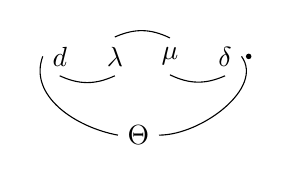
\begin{tikzpicture}
\node (d) at (0,0) {$d$};\node (l) at (.7,0) {$\lambda$};
\node (m) at (1.4,0) {$\mu$};\node (s) at (2.1,0) {$\delta$};
\node (o) at (1,-1) {$\Theta$};\fill (2.4,0) circle (1pt);
\draw (l.north) to[bend left=25] (m.north);

\draw (d.south) to[bend right=25] (l.south);
\draw (m.south) to[bend right=25] (s.south);
\draw (d.west) .. controls (-.4,-.5) and (.2,-.9) .. (o.west);
\draw (s.east) .. controls (2.6,-.4) and (1.8,-1) .. (o.east);
\end{tikzpicture}}
\[
\frac{n(n-1)}2=\frac{5\cdot4}2=10
\qquad\frac{n(n\unsure{-|+}1)}2=\unsure{15|45|q}
\]
\[
d\ \delta\ \lambda\ \overset{i\ge\unsure{1|4}}{\mu_i}\ \Theta
\]
\[
\left\{\begin{aligned}
d^2=\delta^2=\lambda^2&=0\\
\mu_i\mu_j&=C_{ij}\mu_{i+j}
\end{aligned}\right.
\qquad\Theta^2\quad\text{\unsure{rien au dessus|rien à dire}}
\]
\[
d,\delta,\lambda
\]
\[
\hbox{\begingroup\setbox0=\hbox{$\displaystyle \begin{array}{ll}\delta(\unsure{\overline T|T}^{(i)})=0&\\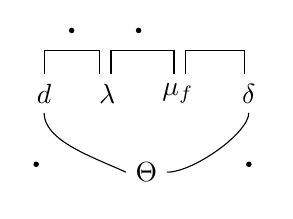
\begin{tikzpicture}[baseline=0pt]
\node (d) at (0,0) {$d$};\node (l) at (.8,0) {$\lambda$};
\node (m) at (1.7,0) {$\mu_f$};\node (s) at (2.6,0) {$\delta$};
\node (o) at (1.3,-1) {$\Theta$};
\draw (0,.25)--(0,.55)--(.7,.55)--(.7,.25);
\draw (.85,.25)--(.85,.55)--(1.65,.55)--(1.65,.25);
\draw (1.8,.25)--(1.8,.55)--(2.55,.55)--(2.55,.25);
\fill (.35,.8) circle (1pt);\fill (1.2,.8) circle (1pt);
\draw (d.south) .. controls (0,-.6) and (.6,-.8) .. (o.west);
\draw (s.south) .. controls (2.6,-.5) and (1.9,-1) .. (o.east);
\fill (-.1,-.9) circle (1pt);\fill (2.6,-.9) circle (1pt);
\end{tikzpicture}&\left\{\begin{aligned}&\overset{\bullet}{d^2}=\delta^2=\overset{\bullet}{\lambda^2}=0\\&\bullet\ \mu_{fg}=\mu_g\mu_f=\unsure{\mu_f\mu_g|\mu_g\mu_f|\mu_{f\prime}=f\prime\mu_1}\\&\Theta^2=-\end{aligned}\right.\end{array}$}\dimen0=\wd0\advance\dimen0 by16pt\divide\dimen0 by2\dimen2=\ht0\advance\dimen2 by\dp0\advance\dimen2 by16pt\divide\dimen2 by2\dimen4=\ht0\advance\dimen4 by-\dp0\divide\dimen4 by2\vrule width0pt height\dimexpr\ht0+10pt\relax depth\dimexpr\dp0+10pt\relax\kern8pt\rlap{\begin{tikzpicture}[overlay,x=1pt,y=1pt,baseline=0pt]\draw (-8pt,\the\dimexpr\ht0+3pt\relax)--(\the\dimexpr\wd0+5pt\relax,\the\dimexpr\ht0+10pt\relax)--(\the\dimexpr\wd0+7pt\relax,\the\dimexpr\ht0+7pt\relax);\draw (-8pt,\the\dimexpr\ht0-6pt\relax)--(-5pt,\the\dimexpr-\dp0-8pt\relax)--(\the\dimexpr.55\wd0\relax,\the\dimexpr-\dp0-4pt\relax);\draw (\the\dimexpr.56\wd0\relax,\the\dimexpr-\dp0-7pt\relax)--(\the\dimexpr\wd0+7pt\relax,\the\dimexpr-\dp0-3pt\relax);\end{tikzpicture}}\box0\kern8pt\endgroup}
\]
\[
\unsure{\varphi|\Phi|\Theta}(\lambda x)=(\deg x+i)\lambda x
\]
\[
\lambda(\unsure{\varphi|\Phi|\Theta} x)=\deg x\ \lambda x
\]
\[
\unsure{\varphi|\Phi|\Theta}\lambda-\lambda\unsure{\varphi|\Phi|\Theta}=i\lambda x
\]
\[
\overset{A}{\sum}\lambda^\epsilon\cdot
\mu_{f(\epsilon,}\ ;\ \delta^{\epsilon'}\Theta-
\]
\[
\hbox{\begingroup\setbox0=\hbox{$\displaystyle d\delta+\delta d=\Theta$}\dimen0=\wd0\advance\dimen0 by16pt\divide\dimen0 by2\dimen2=\ht0\advance\dimen2 by\dp0\advance\dimen2 by16pt\divide\dimen2 by2\dimen4=\ht0\advance\dimen4 by-\dp0\divide\dimen4 by2\vrule width0pt height\dimexpr\ht0+10pt\relax depth\dimexpr\dp0+10pt\relax\kern8pt\rlap{
\begin{tikzpicture}[overlay,x=1pt,y=1pt,baseline=0pt]\draw (-4pt,\the\dimexpr-\dp0-4pt\relax)--(-4pt,\the\dimexpr\ht0+4pt\relax)--(\the\dimexpr\wd0+4pt\relax,\the\dimexpr\ht0+4pt\relax)--(\the\dimexpr\wd0+4pt\relax,\the\dimexpr-\dp0\relax);\draw (-4pt,\the\dimexpr-\dp0-4pt\relax)--(\the\dimexpr\wd0+1pt\relax,\the\dimexpr-\dp0-4pt\relax);\end{tikzpicture}}\box0\kern8pt\endgroup}
\]
\[
\left\{\begin{aligned}
\delta\lambda+\lambda\delta&=\mu_{\unsure{T|\overline T}}\\
d\mu_f-\mu_f d&=\mu_{f'}\lambda\quad\bullet\\
\Theta\lambda-\lambda\Theta&=\lambda\quad\bullet\\
\Theta\mu_f-\mu_f\Theta&=\mu_{\Theta f}\quad\bullet
\end{aligned}\right.
\]
\margin{$\delta(\overline T)=1$}
\[
\sum_{\deleted{\substack{\unsure{\alpha,\beta,\sigma\in\{0,1\}}\\\unsure{n\in\mathbf N}}}}
\underbrace{\mu_{f_{\alpha,\beta,\sigma,}}\lambda^\alpha d^\beta\delta^\sigma\Theta^n}_{
f_{\epsilon,\epsilon',\epsilon'',n}\lambda^\epsilon d^{\epsilon'}\delta^{\epsilon''}\Theta^n}
\]
\margin{$\alpha,\beta,\sigma\in\mathbb F_2$\quad $n\in\mathbf N$}
\[
\deleted{\unsure{\mu_f^\lambda|\mu_f}}
\]
\[
f\lambda^\alpha d^\beta\delta^\sigma\Theta^n
g\lambda^{\alpha'}d^{\beta'}\delta^{\sigma'}\Theta^{n'}
\]
\[
\lambda^\alpha\underset{g d^\beta+\beta g'\lambda}{\hbox{\begingroup\setbox0=\hbox{$d^\beta g$}\vrule width0pt height\ht0 depth\dimexpr\dp0+5pt+\pgflinewidth\relax\rlap{\begin{tikzpicture}[overlay,x=1pt,y=1pt,baseline=0pt]\draw (\the\dimexpr-\pgflinewidth/2\relax,\the\dimexpr-\dp0-\pgflinewidth/2-2pt\relax)--(\the\dimexpr-\pgflinewidth/2\relax,\the\dimexpr-\dp0-\pgflinewidth/2-5pt\relax)--(\the\dimexpr\wd0+\pgflinewidth/2\relax,\the\dimexpr-\dp0-\pgflinewidth/2-5pt\relax)--(\the\dimexpr\wd0+\pgflinewidth/2\relax,\the\dimexpr-\dp0-\pgflinewidth/2-2pt\relax);\end{tikzpicture}}\box0\endgroup}}\delta^\sigma\lambda^{\alpha'}d^{\beta'}\delta^{\sigma'}
\]
Cas $p$ quelconque\inserted{$\ge1$}, $q=1$
\diagram{\begin{tikzcd}[column sep=large,row sep=large]
0\arrow[r,dash]&\Gamma^p\Phi_{\unsure{*|\alpha}}\arrow[r]
&\Gamma^{p}\Phi_{\unsure{*|\alpha}}\otimes\Phi_{\unsure{*|\alpha}}\arrow[r,dash]
&\Gamma^{p}\Phi_{\unsure{*|\alpha}}\otimes\Psi_{\unsure{*|\alpha}}\arrow[r]
\arrow[l,bend left=35,"?",swap]&0\\
&&&\Phi_\alpha\times\Psi_\alpha\arrow[ul]&
\end{tikzcd}}
\diagram{\begin{tikzcd}
\Gamma^{\deleted{\unsure{p}}\inserted{*}+}\Phi_*\otimes\Lambda^{\deleted{\unsure{q|\epsilon}}\inserted{*}}\Psi_*\arrow[d]\\
\Gamma^{*+}\Phi_*\otimes\Lambda^*\Phi_*
\end{tikzcd}}
\[
(\varphi,\psi)\longrightarrow s(\varphi\otimes\psi)\varphi^{(p-1)}
\]
\[
\overset{\deleted{\unsure{q_1|q}}}{\varphi}_1^{(p_1)}-\varphi_r^{(p_r)}\qquad\sum p_i=p
\]
\diagram{\begin{tikzcd}[row sep=large]
\phantom{\varphi_1^{(p_1)}}\arrow[d,mapsto]\\
\phantom{f(\varphi)}
\end{tikzcd}}
\[
\deleted{\sum\lambda_i\unsure{\varphi_i|\varphi}}
\]
\[
\begin{aligned}
f\Bigl(\sum_1^r\lambda_i\varphi_i\Bigr)
&=s\Bigl(\sum\lambda_i\varphi_i\otimes\psi\Bigr)
\Bigl(\sum\lambda_i\varphi_i\Bigr)^{(p-1)}\\
&=\sum_{1\le i\le r}\lambda_i s(\varphi_i\otimes\psi)
\sum_{\substack{(p_1-p_r)\in\mathbf N^r\\\sum p_i=p-1}}
\lambda_1^{p_1}-\lambda_r^{p_r}\varphi_1^{(p_1)}-\varphi_r^{(p_r)}\\
&=\sum_{\substack{1\le i\le r\\(p_1-p_r)}}
\deleted{\unsure{\lambda_i|\lambda_i^2}}\lambda_1^{p_1}\inserted{\lambda_i^{\unsure{\delta_{im}|\delta_{i1}}}}-\lambda_r^{p_r}
s(\varphi_i\otimes\psi)\varphi_1^{(p_1)}-\varphi_r^{(p_r)}
\end{aligned}
\]
\[
\varphi_1^{(q_1)}-\varphi_r^{(q_r)}\longmapsto
\sum_{\substack{\deleted{\substack{\unsure{1\le i\le r}\\\unsure{1\le\alpha\le r}\\\unsure{q_\alpha\ge1}}}\\\inserted{\alpha\in\unsure{\{1-r\}|1-r}}}}
s(\varphi_\alpha\otimes\psi)\varphi_1^{(q_1)}\cdot
\varphi_\alpha^{(q_\alpha-1)}-\varphi_r^{(q_r)}
\]
\[
q_1+-+q_r=p
\]
\diagram{\begin{tikzcd}[row sep=large]
0\\
\Gamma^2\Phi_*\otimes\Psi_*\arrow[u]\arrow[d,bend left=35,"?"]\\
\Gamma^2\Phi_*\otimes\Phi_*\arrow[u]\\
\Gamma^2\Phi_*\arrow[u]\\
0\arrow[u]
\end{tikzcd}}
\diagram{\begin{tikzcd}[row sep=large]
\phantom{\Gamma^q(\Phi)}\\
\Gamma^q(\Phi)\otimes\unsure{\Phi|\Psi}\arrow[u]\arrow[d]\\
\Gamma^q(\Phi)\otimes\Psi
\end{tikzcd}}
\figure{\begin{tikzpicture}\draw (0,0)--(2,2.8);\draw (0,-1.8)--(0,0);\end{tikzpicture}}
\[
\sum_{\alpha\in\{1-r\}.}(\varphi_\alpha\otimes\underset{\displaystyle\sum q_\alpha\psi\varphi_1^{(q_1)}-\varphi_\alpha^{(q_\alpha)}-\varphi_r^{(q_r)}}{\hbox{\begingroup\setbox0=\hbox{$\psi)\varphi_1^{(q_1)}\cdot\varphi_\alpha^{(q_\alpha-1)}-\varphi_r^{(q_r)}$}\vrule width0pt height\ht0 depth\dimexpr\dp0+5pt+\pgflinewidth\relax\rlap{\begin{tikzpicture}[overlay,x=1pt,y=1pt,baseline=0pt]\draw (\the\dimexpr-\pgflinewidth/2\relax,\the\dimexpr-\dp0-\pgflinewidth/2-2pt\relax)--(\the\dimexpr-\pgflinewidth/2\relax,\the\dimexpr-\dp0-\pgflinewidth/2-5pt\relax)--(\the\dimexpr\wd0+\pgflinewidth/2\relax,\the\dimexpr-\dp0-\pgflinewidth/2-5pt\relax)--(\the\dimexpr\wd0+\pgflinewidth/2\relax,\the\dimexpr-\dp0-\pgflinewidth/2-2pt\relax);\end{tikzpicture}}\box0\endgroup}}
\]
\[
\Gamma^p\Phi_*,\quad\Lambda^q\Psi_*,\quad\Lambda^r\Phi_*,
\]
\[
\hbox{\begingroup\setbox0=\hbox{$\displaystyle \Gamma^s\Psi_*\ ?$}\dimen0=\wd0\advance\dimen0 by16pt\divide\dimen0 by2\dimen2=\ht0\advance\dimen2 by\dp0\advance\dimen2 by16pt\divide\dimen2 by2\dimen4=\ht0\advance\dimen4 by-\dp0\divide\dimen4 by2\vrule width0pt height\dimexpr\ht0+10pt\relax depth\dimexpr\dp0+10pt\relax\kern8pt\rlap{\begin{tikzpicture}[overlay,x=1pt,y=1pt,baseline=0pt]\draw (\the\dimexpr\wd0/2\relax,\the\dimen4) ellipse[x radius=\the\dimen0,y radius=\the\dimen2];\end{tikzpicture}}\box0\kern8pt\endgroup}
\]
\[
\delta(\psi\varphi_1^{(q_1)}-\varphi_{\unsure{r|n}}^{(q_{\unsure{r|n}})})
\]
\[
\Phi_*,\Psi_*
\]
\[
\left\{\begin{aligned}
\Gamma^p\Phi_*\otimes\Lambda^q\Psi_*&=\mathscr{DR}_*^{\unsure{pq|p,q}}\\
\Lambda^r\Phi_*&=C_*^{r,0}
\end{aligned}\right.
\]
\mspage{347}
